\documentclass[../main.tex]{subfiles}
\graphicspath{{\subfix{../images/}}}

\begin{document}
To start off easy, we'll cover some problems that involve results - some of which even you'll be able to come up with it! In any case, the main takeaway should be that \textit{understanding} results can help motivate your approaches. That is why thinking triumphs brainless practice!

\begin{figure}[H]
    \centering
    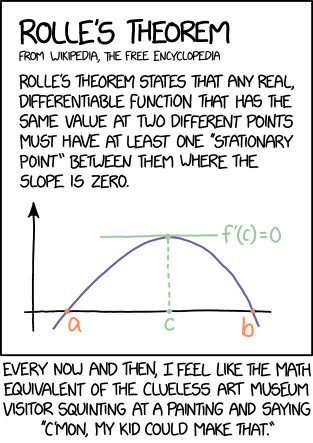
\includegraphics[scale=0.5]{xkcd_rolles_theorem.png}
    \caption{Comic from https://xkcd.wtf/2042/}
\end{figure}

\subsection{Two Classical Results}
We start off with a motivating pursuit curve setup that captures a classic calculus result. Solving the differential equation is defered to the end of the chapter as an exercise.
\begin{example}[2021 H2 Further Math P1 Q11]
At noon, ship $P$ sets sail from port $O$ at a constant speed $V ms^{-1}$ in pursuit of ship $S$ which is travelling due north at constant speed $U ms^{-1}$, where $U < V$. At noon, $S$ is $D$ metres due east of $O$.

$P$ is always steered slightly towards $S$, so that its instantaneous direction is tangential to its \textit{pursuit-curve}, as shown in the diagram.

Write down:
\begin{itemize}
    \item the coordinates for $S$ at time $t$ after noon, and
    \item an expression for $\frac{dy}{dx}$.
\end{itemize}
\end{example}
\begin{figure}[H]
    \centering
    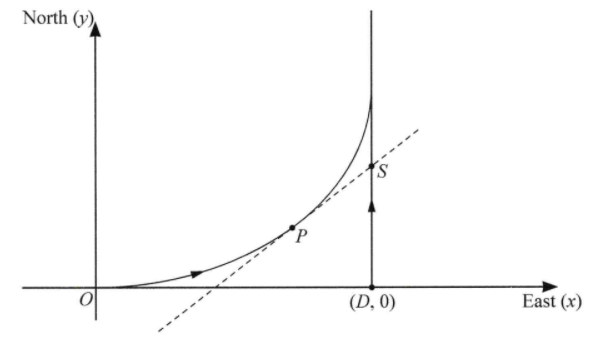
\includegraphics{graph-pursuit.PNG}
    \caption{The pursuit curve of $P$}
    \label{fig:graph-pursuit}
\end{figure}
Since $S$ moves at a constant speed $U$ vertically, the coordinates of $S$ at time $t$ is simply $(D, Ut)$. 

Moreover, $\frac{dy}{dx}$ is the gradient of the tangent at $P$, as drawn. In other words, $\frac{dy}{dx}$ is simply the gradient of the line $PS$. Since $P$ lies on the curve, $P$ has coordinates $(x, y)$. Hence,
\begin{equation} \label{2.1-gradient}
    \frac{dy}{dx}=\frac{Ut-y}{D-x}
\end{equation}
Here, we have $D-x > 0$ since the path of $P$ approaches the path of $S$ (we don't discuss the case $D=x$, since this corresponds to the point where the two curves intersect). In this case, it should be noted that the path for $S$ is an asymptote for the path of $P$.  
\begin{example}[cont.]\label{pursuit-curve:results}
Let $m=\frac{dy}{dx}$. Explain why, with reference to the distance travelled by $P$, $\frac{d}{dx}(Vt)=\sqrt{1+m^2}$.

Using all of these results, show that $(D-x)\frac{dm}{dx}=\lambda\sqrt{1+m^2}$ where $\lambda=\frac{U}{V}$
\end{example}
First, we should be convinced that our expressions as above are right. Seeing that the term $(D-x)$ appears in the denominator of \eqref{2.1-gradient}, and that it also appears in the second equation that is demanded of us in this part, we are reassured that we are on the right track.

Two things now jump out to us: firstly, why the derivative with respect to $x$? What does $Vt$ represent, and where does $\sqrt{1+m^2}$ come from?

Some students may notice that this form resembles the arc length formula, and that the arc length of an explicit curve from $x=a$ to $x=b$ is given by
$$\int_{a}^{b}\sqrt{1+\left(\frac{dy}{dx}\right)^2} \,dx =\int_{a}^{b}\sqrt{1+m^2} \,dx .$$
Since the question guides us to consider the distance travelled by $P$, we note that this can be given by the arc length from $u=0$ to $u=x$ (note the change in variable names!). Furthermore, $V$ is defined as the speed of ship $P$. Thus, the total distance travelled by $P$ is simply $Vt$, and this is equal to the arc length:
$$Vt=\int_{0}^{x}\sqrt{1+m^2} \,du$$

Next, we need to resolve the derivative - where does it come from? The presence of the derivative can only mean one thing! Recall the Fundamental Theorem of Calculus (which every student conveniently sees in the lecture notes and then promptly forgets), which says that: 
\begin{theorem}[Fundamental Theorem of Calculus]
Let $f$ be a continuous (real) function defined on the closed interval $[a,b]$. Let $F(x)$ defined for all $x\in[a,b]$ by:
$$F(x)=\int_a^x f(u)\,du,$$ then $$F'(x)=f(x)$$ for all $x \in (a, b)$. 
\end{theorem}
By applying this to the problem at hand, we have, for the choice $a=0$:
\begin{equation}\label{2.1-distance}
    \frac{d}{dx}(Vt)=\sqrt{1+m^2}
\end{equation}

To address the second part, we first see that \eqref{2.1-distance} immediately implies $$V\frac{dt}{dx}=\sqrt{1+m^2}.$$ Further, the term $\frac{dm}{dx}=\frac{d}{dx}\frac{dy}{dx}$ strongly suggests that we differentiate \eqref{2.1-gradient}. We have:
\begin{align*}
    (D-x)\frac{dy}{dx}=Ut-y &\Longrightarrow (D-x)m = Ut-y \\
    &\Longrightarrow (D-x)\frac{dm}{dx}-m=U\frac{dt}{dx}-m \\
    &\Longrightarrow (D-x)\frac{dm}{dx}=U\frac{dt}{dx} \\
    &\Longrightarrow (D-x)\frac{dm}{dx}=\frac{U}{V}\sqrt{1+m^2}=\lambda\sqrt{1+m^2}.
\end{align*}
Finally, we note again that since $D-x > 0$, $\lambda\sqrt{1+m^2} \neq 0$, so $\lambda$ is non-zero, and the setup holds.  

\begin{moral}
This question is not hard in terms of the technical demands, but it is the first of many problems in this handout that places due emphasis on recognition.
\end{moral}

The next example showcases a classic puzzle that involves a special case of the cubic discriminant(!), as well as another classic calculus result that helps motivate our approach.
\begin{example}
Given that $y=mx+c$ is a tangent to the curve $y=x^3$, show that 
$$27c^2=4m^3.$$
\end{example}
You may be tempted to immediately pull out the quadratic discriminant, but not so fast! This setup introduces the unfamiliar cubic, so you either regurgitate the cubic discriminant (no!!!) or come up with something innovative...

We could begin by differentiating, so $m=\frac{dy}{dx}=3x^2$ for each point $(x,y)=(a,a^3)$ for any choice of $a \in \mathbb{R}$. Thus, the tangent at this point has equation $y-a^3=3a^2(x-a) \Longrightarrow y=3a^2x-2a^3$, and by a direct comparison, $m=3a^2$ and $c=-2a^3$.
Finally, we make short work of this setup: $27c^2=108a^6=4m^3$, as required.

It's not often that our first approach works, but I'm still not very satisfied by this solution: it doesn't tell us anything about the geometric setup...

Perhaps we can make a rough sketch:
\begin{figure}[H]
    \centering
    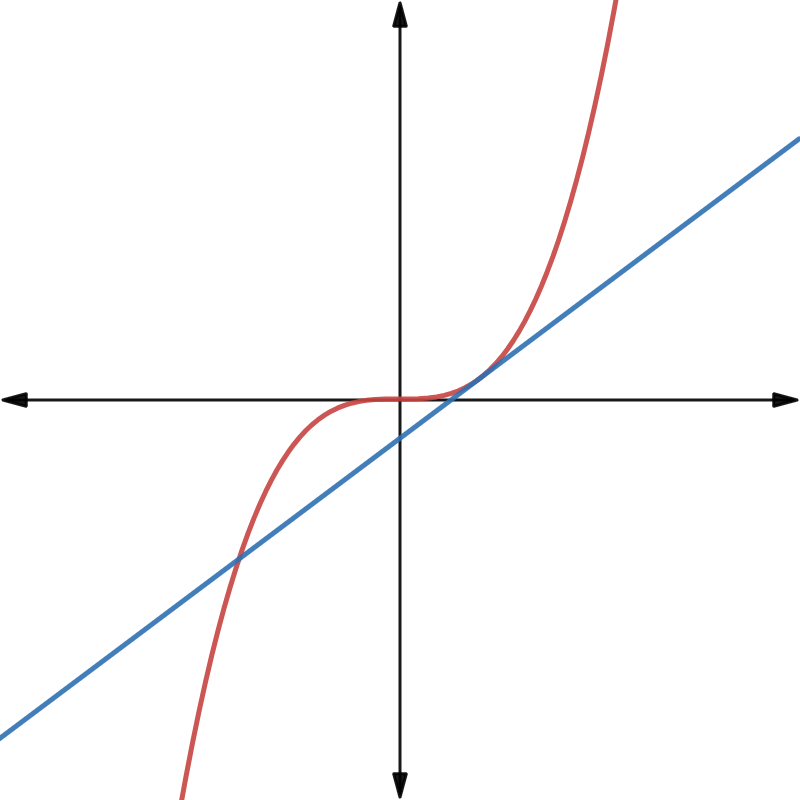
\includegraphics[scale=0.25]{graph-cubic-tangent.PNG}
    \caption{Tangent to $y=x^3$}
    \label{fig:graph-cubic-tangent}
\end{figure}
Certainly, we should note that a tangent still intersects the cubic at 2 distinct points (we do not discuss the "tangent" at $x=0$ because it isn't exactly a tangent). This means that the equation $x^3=mx+c$ has 2 distinct solutions.

But wait! Shouldn't a cubic polynomial (with real coefficients) have 3 complex solutions? Since we concluded that there are exactly 2 distinct, and in particular, real solutions, that means the third one must also be real (why?).

Hence, one of the roots to the equation is a \textbf{double root}. In fact, the double root occurs at the point of tangency (also, why?). We now write:
$$x^3-mx-c=(x-a)^2(x-b)=x^3-(2a+b)x^2+(a^2+2ab)x-a^2b.$$
Thus, we have $c=-2a^3$ and $m=3a^2$ and we may finish off as above.
\begin{example}[cont.]
It is given that the cubic $x^3=mx+c$ has three distinct roots. By using a sketch, explain why
$$27c^2<4m^3.$$
\end{example}
The setup is slightly different: it is now given that the cubic has three distinct roots instead of the two that we found above! Thus, the line $y=mx+c$ is a \textbf{secant} to the curve $y=x^3$. However, the conclusion is still very suspiciously similar: it is just the equality sign being replaced by the $<$ sign. In some way, this suggests that a tangent is still in play... somewhere...

Furthermore, we are guided to use a sketch. Perhaps we should play around with a few sketches to find some foothold.
\begin{figure}[H]
    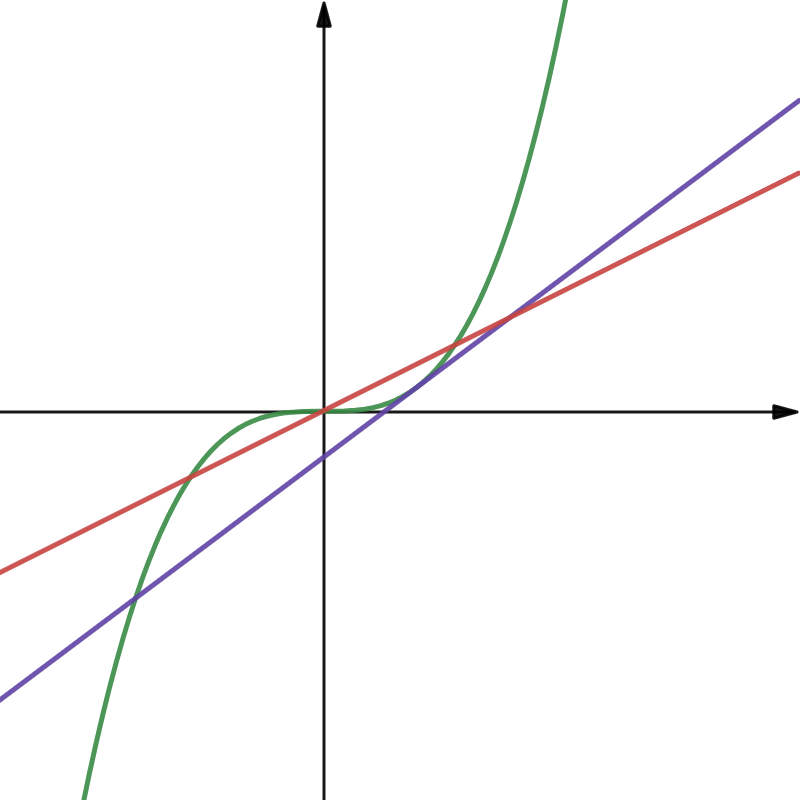
\includegraphics[width=0.3\textwidth]{graph-cubic-lowslant-secant.png}
    \hfill
    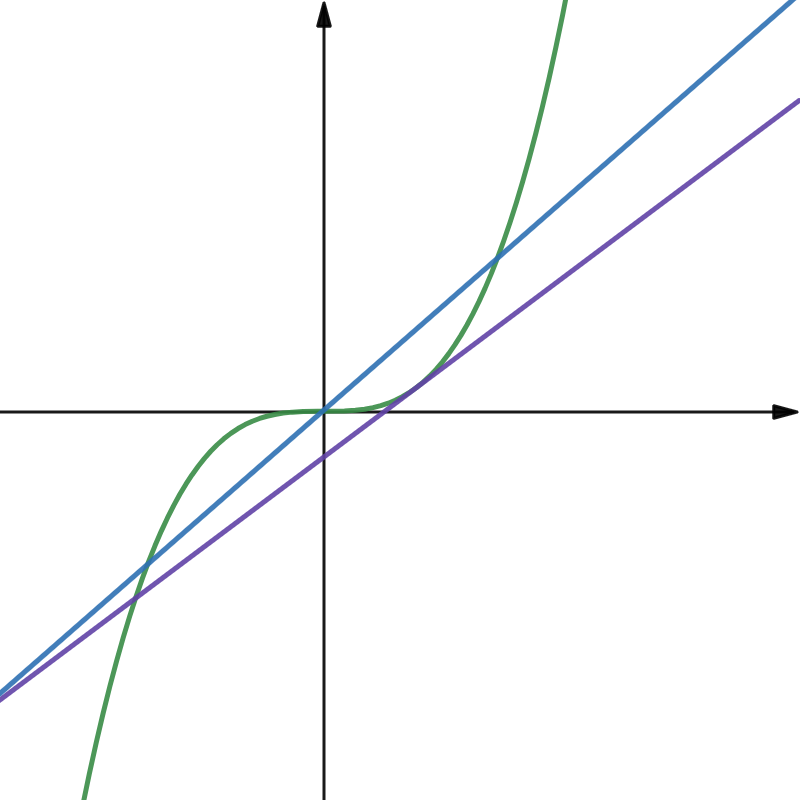
\includegraphics[width=0.3\textwidth]{graph-cubic-highslant-secant.png}
    \hfill
    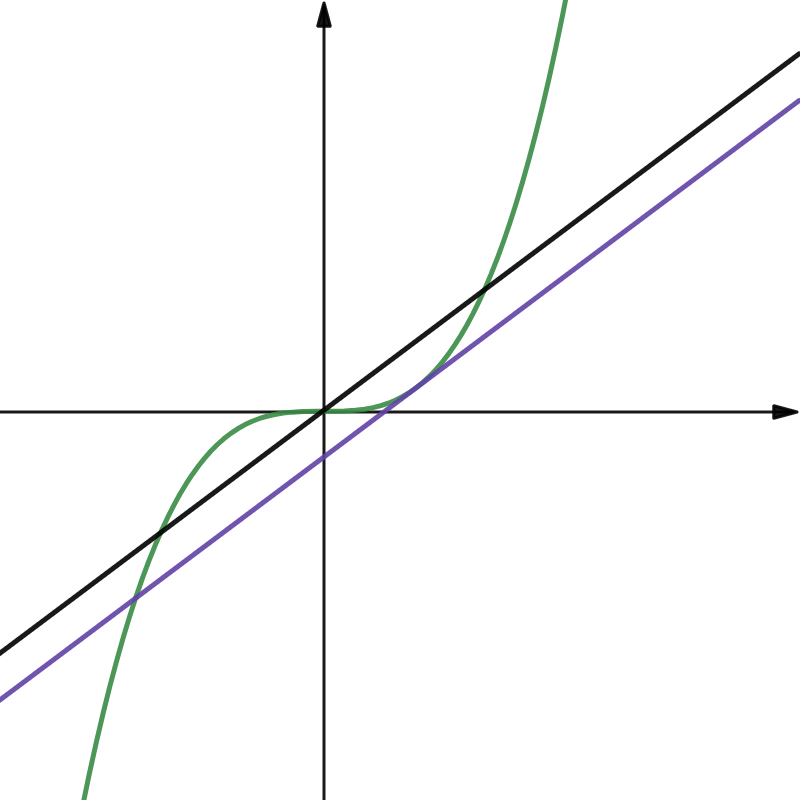
\includegraphics[width=0.3\textwidth]{graph-cubic-parallel-secant.png}
    \caption{Setups with secants having various gradients}
\end{figure}
Some thought would lead you to think that the secant that is parallel to the tangent would be most promising to consider. Indeed, $c^2$ and $m^3$ are both directly related to the intercepts of the tangent, and $c=-2a^3$ represents the y-intercept of the line in question. Perhaps we should dig into the intercepts of the secant in the third sketch.

As a matter of fact, we should be somewhat wary of such a claim. While in this case, our sketch tells us that there exists a secant to the cubic curve that is parallel to a given tangent, this is not immediately obvious for any other curve! However, we are reassured by a well-known calculus result!

\begin{theorem}[Mean Value Theorem]
If $f$ is a continuous function on $[a,b]$ and differentiable on $(a,b)$, then there exists a point $c \in (a,b)$ such that
$$f'(c)=\frac{f(b)-f(a)}{b-a}.$$
\end{theorem}
Loosely speaking, between two points on a smooth curve, there exists at least one point such that the tangent to that point is parallel to the secant passing through these two points.

Suppose $c$ is the y-intercept of the tangent to the cubic, and let $c'$ be the y-intercept of the secant. In the diagram, we have $c' > c$. Certainly, if our secant lies underneath the tangent, then we only get 1 intersection. Moreover, our secant cannot lie "too far away" from the origin. More rigorously, we cannot have $|c|<|c'|$ since $|c'|$ is the distance from the secant to the origin, and we know that this distance can't be larger than $|c|$, which is the distance from the tangent to the origin (or otherwise, we only get 1 intersection).

Thus, we must have $|c'|<|c| \Longrightarrow 27(c')^2 < 27c^2 = 4m^3$ by using the result proven above.

\begin{example}[cont..]
A circle passes through the origin and has four distinct intersections with the parabola $y=x^2$. Describe the possible positions of the centre of the circle.
\end{example}
This question looks innocuously simple to deal with algebraically, so let's proceed algebraically first. Let the circle have equation $(x-a)^2+(y-b)^2=r^2$, with radius $r^2=a^2+b^2$. Apparently, the condition of "four distinct intersections" is enough for us to describe the entire set of possible centres...

For intersections, we need
\begin{align*}
    &(x-a)^2+(y-b)^2 =(x-a)^2+(x^2-b)^2=r^2 \\
    \Longleftrightarrow& \,x\left[x^3-(2b-1)x-2a\right]=0\\
\end{align*}
At this step, one of the roots is $x=0$, which confirms the problem statement that the circle passes through the origin. Hence, one of the four intersections is at the origin. The other three is given by the cubic equation 
\begin{equation}\label{2.9-cubic}
    x^3=(2b-1)x+2a.
\end{equation} A cursory look would remind us \eqref{2.9-cubic} represents the intersections between the curve $y=x^3$ and the line $y=(2b-1)x+2a$. Thus, we should use the part above to determine a \textbf{necessary and sufficient} condition so that this cubic equation has exactly 3 distinct roots.

At the end, we should remember to check that $x=0$ is \textit{not} a solution of this cubic, otherwise we will only have 3 distinct roots in total. We first proceed with the choice $m=2b-1, c=2a$, and we have $$27(2a)^2 < 4(2b-1)^3 \Longleftrightarrow b > \frac{1}{2}\left(3a^{\frac{2}{3}}+1\right).$$

Finally, we work towards excluding $x=0$. If $x=0$ is a solution to the cubic, then $2a=0$, and it becomes clear that we must exclude $a=\frac{1}{2}$ (otherwise, we only have three distinct intersections instead of four).

Moreover, we also need $b > 0$, otherwise we get at most 2 solutions (graph this!). Yet, we are fortunate enough: since $b > \frac{1}{2}\left(3a^{\frac{2}{3}}+1\right) > \frac{1}{2}\cdot 1 = \frac{1}{2} > 0$.

Now, to formally write the proof in the \textit{forwards direction}.
\begin{proof}
Let the equation of the circle be $(x-a)^2+(y-b)^2=a^2+b^2$.
For intersections with the parabola $y=x^2$, we have
\begin{align*}
    &(x-a)^2+(y-b)^2 =(x-a)^2+(x^2-b)^2=r^2 \\
    \Longleftrightarrow& \,x\left[x^3-(2b-1)x-2a\right]=0,\\
\end{align*}
and so the intersections occur at $x=0$ and at the three distinct roots of 
$$x^3=(2b-1)x+2a.$$
From the above result, the choice $m=2b-1, c=2a$ yields that $$27(2a)^2 < 4(2b-1)^3 \Longleftrightarrow b > \frac{1}{2}\left(3a^{\frac{2}{3}}+1\right).$$
Moreover, we must have $a \neq \frac{1}{2}$, otherwise $x=0$ is a solution to the cubic, and we also have $b > 0$. 

Hence, the set of all possible centres is the set 
$$\left\{(a,b): b > \frac{1}{2}\left(3a^{\frac{2}{3}}+1\right), a\neq \frac{1}{2}, a \in \mathbb{R}\right\}.$$
\end{proof}

In fact, we are guaranteed that two conics intersect at at most four points:
\begin{theorem}[Bezout's Theorem on Intersection Points]
Suppose that $X$ and $Y$ are two plane curves that are not multiples of each other. Then the total number of intersection points of X and Y counted with their multiplicities (including complex intersections and points at infinities), is equal to the product of the degrees of X and Y.
\end{theorem}

\begin{moral}
This problem is slightly more demanding in terms of finding a good starting point, and emphasises that having good diagrams should be a major part of anyone's problem solving toolkit.
\end{moral}

This final worked example showcases the challenges of generalising the quotient rule.
\begin{example}[part 2021 H3 Math P1/3]\label{generalised-quotient-rule:p1}
Let $u$ and $v$ be quadratic functions of $x$ and let $y=\frac{u}{v}$. It is known that for $n\in \mathbb{Z}^+,$
$$v\frac{d^{n+2}y}{dx^{n+2}}+(n+2)\frac{dv}{dx}\frac{d^{n+1}y}{dx^{n+1}}+\binom{n+2}{2}\frac{d^{2}v}{dx^{2}}\frac{d^n{y}}{dx^{n}}=0.$$

Now suppose that $v=(\alpha-x)^2$ for some real $\alpha$ and, for all positive integers $n$, define
$$z_n=\frac{(\alpha-x)^{n+2}}{n!}\frac{d^{n}y}{dx^{n}}.$$
Prove that $\{z_n\}$ is an arithmetic progression.
\end{example}
\begin{remark}
The given identity can be proven by induction. We omit this part because it involves only uninspiring algebraic manipulations. The proof is defered to the Selected Problems section
\end{remark}
To start us off, we note that $z_n$ contains $n!$ in their denominator, but no term in the given result does. Moreover, $$\binom{n+2}{2}=\frac{(n+2)(n+1)}{2},$$ so we are motivated to divide throughout by $(n+2)!$:
\begin{align*}
    \frac{v}{(n+2)!}\frac{d^{n+2}y}{dx^{n+2}}+\frac{1}{(n+1)!}\frac{dv}{dx}\frac{d^{n+1}y}{dx^{n+1}}+\frac{1}{2(n!)}\frac{d^{2}v}{dx^{2}}\frac{d^n{y}}{dx^{n}}=\frac{v}{(n+2)!}\frac{d^{n+2}y}{dx^{n+2}}-2\frac{(\alpha-x)}{(n+1)!}\frac{d^{n+1}y}{dx^{n+1}}+\frac{1}{n!}\frac{d^n{y}}{dx^{n}}=0
\end{align*}
(Note the 1-2-1 symmetry in the coefficients, this tells us something is right!) Now, we proceed as per normal. We have
\begin{align*}
    z_{n+1}-z_{n}&=\frac{(\alpha-x)^{n+3}}{(n+1)!}\frac{d^{n+1}y}{dx^{n+1}}-\frac{(\alpha-x)^{n+2}}{n!}\frac{d^ny}{dx^n}\\
    &=(\alpha-x)^{n+2}\left(\frac{(\alpha-x)}{(n+1)!}\frac{d^{n+1}y}{dx^{n+1}}-\frac{1}{n!}\frac{d^ny}{dx^n}\right) = (\alpha-x)^{n+2}\left(\frac{v}{(n+2)!}\frac{d^{n+2}y}{dx^{n+2}}-\frac{(\alpha-x)}{(n+1)!}\frac{d^{n+1}y}{dx^{n+1}}\right)\\
    &=\frac{(\alpha-x)^{n+4}}{(n+2)!}\frac{d^{n+2}y}{dx^{n+2}}-\frac{(\alpha-x)^{n+3}}{(n+1)!}\frac{d^{n+1}y}{dx^{n+1}} = z_{n+2}-z_{n+1}
\end{align*}
for all $n$. (Note also the 1-2-1 symmetry here!) Since consecutive differences are equal for all $n$, this difference must be independent of $n$, and hence the sequence is arithmetic, with common difference $z_{n}-z_{n-1}=z_{n-1}-z_{n-2}=\cdots=z_2-z_1$.

With a bit of foresight, we say that the common difference is $z_2-z_1.$
\begin{example}[cont.]
By writing $y$ as partial fractions, show that the common difference is $u(\alpha)$.
\end{example}
It is finally time to see what $u$ has to bring... We first write $u(x)=Ax^2+Bx+C = A(x^2-2\alpha x+\alpha^2)+(B+2A\alpha)x+(C-A\alpha^2)$ so that
$$y=\frac{u}{v}=A+\frac{(B+2A\alpha)x+(C-A\alpha^2)}{(\alpha-x)^2}=A+\frac{D}{\alpha-x}+\frac{E}{(\alpha-x)^2}.$$
By expanding, we have:
\begin{align*}
    (B+2A\alpha)x+(C-A\alpha^2)=D(\alpha-x)+E &\Longrightarrow -D=B+2A\alpha, \, D\alpha+E=C-A\alpha^2 \\
    &\Longrightarrow (-B-2A\alpha)\alpha+E=C-A\alpha^2 \\
    &\Longrightarrow E=A\alpha^2+B\alpha+C
\end{align*}
Hmm... That's peculiar. It turns out that we have E=$u(\alpha)$, and so we should expect that $E$ is indeed the common difference.
It would now be handy to evaluate the derivatives: $$\frac{dy}{dx}=\frac{D}{(\alpha-x)^2}+\frac{2E}{(\alpha-x)^3},\; \frac{d^2y}{dx^2}=\frac{2D}{(\alpha-x)^3}+\frac{6E}{(\alpha-x)^4}.$$

Finally, the common difference is
\begin{align*}
    z_2-z_1&=\frac{(\alpha-x)^4}{2}\frac{d^2y}{dx^2}-(\alpha-x)^3\frac{dy}{dx} \\
    &=D(\alpha-x)+3E-D(\alpha-x)-2E=E,
\end{align*}
as needed.
\begin{moral}
The problem may look unsightly, but it's bark is really worse than it's bite. In approaching lengthy computational problems like these, it is wise to pay attention to special terms that hint to us what we should work with.
\end{moral}
\subsection{Series Expansions}
Most problems on Maclaurin series solve themselves just by using some known series expansions from the formula list. That said, the trickier ones require you to make a judicious choice on the order to apply them, especially since these series are \textit{conditionally convergent}, so we must be careful not to generate an "infinite" number of terms.
\begin{example}[2021 H2 Further Math P1/5b] 
Consider the equation $f(x)=0$ and let $\alpha$ denote the single root, where $f(x)=xe^{x-1}+x-2-\delta$ and $\delta$ is very close to $0$.

Use two iterations of the Newton-Raphson method, with initial approximation $x_0=1$, to show that $\alpha \approx 1+\frac{1}{3}\delta-\frac{1}{18}\delta^2$, where terms in $\delta^3$ and higher powers of $\delta$ have been ignored.
\end{example}
By the Newton-Raphson recurrence, $$x_{n+1}=x_n-\frac{x_ne^{x_n-1}+x-2-\delta}{(1+x_n)e^{x_n-1}+1}.$$
Now, the presence of the fraction makes our approach clear: either we begin by substituting for $e^{x_n}$, or by considering $\left[(1+x_n)e^{x_n-1}+1\right]^{-1}$

Suppose that we started with taking the reciprocal by assuming the binomial expansion holds, then we would have:
\begin{align*}
    x_1 &= 1+\frac{\delta}{3}\\
    x_2 &= 1+\frac{\delta}{3}-\frac{\left(1+\frac{\delta}{3}\right)e^{\frac{\delta}{3}}-1-\frac{2\delta}{3}}{\left(2+\frac{\delta}{3}\right)e^\frac{\delta}{3}+1} \\
    &= 1+\frac{\delta}{3}-\left[\left(1+\frac{\delta}{3}\right)e^{\frac{\delta}{3}}-1-\frac{2\delta}{3}\right]\left[1+m+\frac{m^2}{2}+\cdots\right]
\end{align*}
where $m=\left(2+\frac{\delta}{3}\right)e^\frac{\delta}{3}$.

Now, we attempt to simplify the second square bracket by using the Maclaurin expansion for $e^x:$
\begin{align*}
    m &= \left(2+\frac{\delta}{3}\right)e^\frac{\delta}{3} \\ &= \left(2+\frac{\delta}{3}\right)\left(1+\frac{\delta}{3}+\frac{\delta^2}{18}+\cdots\right) \\
    m^2 &= \left(2+\frac{\delta}{3}\right)^2e^\frac{2\delta}{3} \\ &= \left(2+\frac{\delta}{3}\right)^2\left(1+\frac{2\delta}{3}+\frac{4\delta^2}{18}+\cdots\right) \\
    m^3 &= \left(2+\frac{\delta}{3}\right)^3e^\delta \\ &= \left(2+\frac{\delta}{3}\right)^3\left(1+\delta+\frac{\delta^2}{2}+\cdots\right)\\
    &\cdots
\end{align*}
It is not difficult to see that we immediately have a problem. The terms $m, m^2, m^3, \cdots$ generate infinitely many terms in $\delta^0, \delta^1$ and $\delta^2$, and so this means $\{x_n\}$ diverges to infinity..???. Indeed, it is clear why this fails: the Binomial Expansion for $(1+m+\frac{m^2}{2}+\cdots)^{-1}$ only holds when $f(m)=m+\frac{m^2}{2}+\cdots < 1$, but graphical work shows that $m\approx 2$ for $\delta \approx 0$, so $f(m)$ is certainly not small. 

This means that we should begin with substituting the Maclaurin expansion for $e^x$, then apply the binomial expansion:
\begin{align*}
    x_1 &= 1+\frac{\delta}{3}\\
    x_2 &= 1+\frac{\delta}{3}-\frac{\left(1+\frac{\delta}{3}\right)e^{\frac{\delta}{3}}-1-\frac{2\delta}{3}}{\left(2+\frac{\delta}{3}\right)e^\frac{\delta}{3}+1} \\
    &\approx 1+\frac{\delta}{3}-\frac{\left(1+\frac{\delta}{3}\right)\left(1+\frac{\delta}{3}+\frac{\delta^2}{18}\right)-1-\frac{2\delta}{3}}{\left(2+\frac{\delta}{3}\right)\left(1+\frac{\delta}{3}+\frac{\delta^2}{18}\right)+1} \\
    &\approx 1+\frac{\delta}{3}-\frac{\frac{\delta^2}{6}}{3+\delta+\frac{\delta^2}{6}} =1+\frac{\delta}{3}-\frac{\frac{\delta^2}{18}}{1+\frac{\delta}{3}+\frac{\delta^2}{18}} \\
    &\approx 1+\frac{\delta}{3}-\frac{\delta^2}{18}\left(1+\frac{\delta}{3}+\frac{\delta^2}{18}+\frac{\delta^2}{9}\right) \\ 
    &\approx 1+\frac{\delta}{3}-\frac{\delta^2}{18}
\end{align*}

\paragraph{Tangent: Conditional Convergence}
We say that a series $\{a_n\}$ is \textbf{conditionally convergent} if $\lim_{n\to\infty}\sum a_n$ exists (i.e. the sum converges), but $\lim_{n\to\infty}\sum a_n \to \infty$. For an example, we saw above that the binomial series
$$(1+x)^{\alpha}=\sum_{k=0}^{\infty}\binom{\alpha}{k}x^k$$
is conditionally convergent.

In particular, we saw that by some magical rearrangement, we supposedly see that $x_n$ diverges to infinity. Riemann confirms this:
\begin{theorem}[Riemann's Rearrangement Theorem]
If an infinite series of real numbers is conditionally convergent, then its terms can be arranged in a permutation so that the new series converges to an arbitrary real number, or diverges.
\end{theorem}
Let us investigate the canonical example of the alternating harmonic series:
$$H=1-\frac{1}{2}+\frac{1}{3}-\frac{1}{4}+\cdots=\ln{2}.$$
Suppose we rearrange the terms so that each block of three terms are given by
$$\frac{1}{2k-1}-\frac{1}{2(2k-1)}+\frac{1}{4k},$$
so that 
\begin{align*}
    H_{R}&=\left(1-\frac{1}{2}-\frac{1}{4}\right)+\left(\frac{1}{3}-\frac{1}{6}-\frac{1}{8}\right)+\left(\frac{1}{5}-\frac{1}{10}+\frac{1}{12}\right)+\cdots \\
    &=1-\frac{1}{2}-\frac{1}{4}+\frac{1}{6}-\frac{1}{8}+\frac{1}{10}+\frac{1}{12} +\cdots \\
    &=1-\frac{1}{2}\left(1+\frac{1}{2}-\frac{1}{3}+\frac{1}{4}+\cdots\right) \\
    &=1-\frac{1}{2}\ln{2}
\end{align*}
Of course, this isn't exactly right! But Riemann tells us that any magical rearrangement begets magical results...

\subsection{Integration By Parts}
{Integration By Parts}
Simply follow the divine LIATE rule, right..? Some questions just don't die though... Here's a quick example:
\begin{example}[2021 NYJC H2 Math P1/6b]
Find $\int x\sin{(\ln{x})} \,dx$.
\end{example}
Simple! Let $u=x, dv=\sin{(\ln{x})} \,dx$... How do we integrate $dv$? Maybe we choose $u=\sin{\ln{x}}, dv=x$ instead, but now $v=\frac{x^2}{2}$! Somehow this question goes out of its way to obstruct the rule. 

Let's take a step back, and realise that $\sin{(\ln{x})}$ simply sticks out like a sore thumb. Really: $\ln x$ wrapped inside sine... Maybe we can do this by the most obvious substitution: $u=\ln x, du=\frac{1}{x} \,dx \Longrightarrow \,dx = x\,du$, so that $\int x\sin{(\ln x)} \,dx= \int u^2\sin{u} \,du$. Now this is more friendly to our LIATE rule.

Another example for difficult choices when using integration by parts is in handling reduction formulae: expressing integrals in terms of recurrences.
\begin{example}[Classic]
Letting $$I_n=\int_{0}^{\frac{\pi}{4}}\tan^n x\,dx, n\geq 2,$$
show that $I_n+I_{n-2}=\frac{1}{n-1}$.
\end{example}
A usual choice would be $u=\tan^n x$, $dv=1$ so that
\begin{align*}
    I_n&=\int_{0}^{\frac{\pi}{4}}\tan^n x \,dx = \left[x\cdot \tan^n x\right]_{0}^{\frac{\pi}{4}}-n\int_{0}^{\frac{\pi}{4}}x\cdot \tan^{n-1} x\sec^2x\,dx \\
    &=\frac{\pi}{4}-n\left(\left[\frac{x\cdot \tan^nx}{n}\right]_{0}^{\frac{\pi}{4}}-\int_{0}^{\frac{\pi}{4}}\frac{\tan^nx}{n}\,dx\right) \\
    &=\frac{\pi}{4}-\left(\frac{\pi}{4}-I_n\right) = I_n
\end{align*}
Hmm... This substitution doesn't give us anything new. What else?

For one, our final result contains a term in $I_{n-2}$, thus we should expect to split the integral in such a way that contains either a $tan^{n-1}x$ term which eventually reduces to some term with exponent $n-2$, like $\tan^nx=\tan^{n-1}x\cdot \tan x$; or a term in $\tan^{n-2}x$, like $\tan^n x=\tan^{n-2}x\cdot \tan^2x$.

With a bit of thinking and imagining how both methods will fare, it is clear that the second rearrangement will yield us the most mileage. Indeed, we can see that $\frac{d}{dx}\tan x=\sec^2x=\tan^2x+1$. So, this makes sense:
\begin{align*}
    I_n&=\int_{0}^{\frac{\pi}{4}}\tan^{n-2}x\cdot \tan^2x \,dx \\
    &=\int_{0}^{\frac{\pi}{4}}\tan^{n-2}x\cdot \sec^2x-\tan^{n-2}x \,dx \\
    &=\left[\frac{\tan^{n-1}x}{n-1}\right]_{0}^{\frac{\pi}{4}}-I_{n-2} &&\text{using integration by parts}\\
    &=\frac{1}{n-1}-I_{n-2}
\end{align*}
as needed.

Another reduction formula requires slightly more insight to rewrite:
\begin{example}
Letting 
$$I_n=\int_{0}^{1}\frac{x^n}{\left(1+x^2\right)^3} \,dx, n\geq 2$$
prove that $(5-n)I_n=(n-1)I_{n-2}-\frac{1}{4}$.
\end{example}
With the standard form for $\int f'f^n=\frac{f^{n+1}}{n+1}+C$ in mind, it would be wise to rewrite:
$$I_n=\int_{0}^{1}\frac{x^n}{\left(1+x^2\right)^3} \,dx
    =\frac{1}{2}\int_{0}^1\frac{x^{n-1}\cdot2x}{\left(1+x^2\right)^3} \,dx,$$
    whence the choice $u=x^{n-1}, \,du=(n-1)x^{n-2}$ and $dv=\frac{2x}{(1+x^2)^3} \,dx, v=\frac{(1+x^2)^{-2}}{-2}$ becomes clear.
Thus,
\begin{align*}
    I_n &=\int_{0}^{1}\frac{x^n}{\left(1+x^2\right)^3} \,dx
    =\frac{1}{2}\int_{0}^1\frac{x^{n-1}\cdot2x}{\left(1+x^2\right)^3} \,dx \\
    &=\frac{1}{2}\left(\left[\frac{x^{n-1}}{-2(1+x^2)^2}\right]_{0}^{1}+\frac{n-1}{2}\int_{0}^{1}\frac{x^{n-2}}{(1+x^2)^2}\,dx\right) \\
    &=-\frac{1}{16}+\frac{n-1}{4}\int_{0}^{1}\frac{x^{n-2}(1+x^2)}{(1+x^2)^3}\,dx &&\parbox{5.5cm}{Here we multiplied the numerator and denominator by $(1+x^2)$}\\
    &=-\frac{1}{16}+\frac{n-1}{4}\int_{0}^{1}\frac{x^{n-2}}{(1+x^2)^3}+\frac{x^n}{(1+x^2)^3}\,dx &&\text{splitting terms}\\
    &=-\frac{1}{16}+\frac{n-1}{4}(I_{n-2}+I_n),
\end{align*}
and we get, by rearranging, 
\begin{align*}
    16I_n=-1+4(n-1)(I_{n-2}+I_n) &\Longrightarrow (16-4(n-1))I_n=-1+4(n-1)I_{n-2} \\ &\Longrightarrow (20-4n)I_n=-1+4(n-1)I_{n-2} \\ &\Longrightarrow (5-n)I_n=-\frac{1}{4}+(n-1)I_{n-2}
\end{align*}
Symmetry is perhaps the most useful property in math. In short, we like symmetry because it makes things simple. It is particularly useful in calculations that concern complicated expressions, integrals, identities etc, and identifying and exploiting these symmetries will make algebra clear up easily. Even outside of algebra, geometric and graphical symmetries are always useful.

Our first worked example is a poster problem for just how useful symmetry is.
\begin{example}[Classic]
The Laplace distribution has probability density function
$$f(x)=k\exp{\left(-\frac{|x-\mu|}{b}\right)}, x \in \mathbb{R},$$
where $\mu$ is the location parameter, $b$ is the scale parameter and $k$ is a constant.

Show that $k=\frac{1}{2b}.$
\end{example}
I immediately get a gag reflex whenever I see a modulus sign in integrals, so we immediately separate the regions. The corresponding cases for $x > \mu$ and $x < \mu$. Now, to find $k$, we simply integrate:
\begin{align*}
    1&=\int_{-\infty}^{\infty}f(x) \,dx = \int_{-\infty}^{\infty}k\exp{\left(-\frac{|x-\mu|}{b}\right)} \,dx \\
    &= k\left[\int_{-\infty}^{\mu} \exp{\left(-\frac{\mu-x}{b}\right)}+\int_{\mu}^{\infty}\exp{\left(-\frac{x-\mu}{b}\right)}\,dx \right] \\
    &=k\left(\left[b\exp{\left(\frac{x-\mu}{b}\right)}\right]_{-\infty}^{\mu}+\left[-b\exp{\left(\frac{\mu-x}{b}\right)}\right]_{\mu}^{\infty}\right) \\
    &= 2kb
\end{align*}
Hence, $k=\frac{1}{2b}$.

This is a perfectly viable approach, but on a closer look, it's not hard to see the $f(x)$ is symmetrical about $x=\mu$, simply because of the modulus sign wrapping it. Now, we only need to consider exactly one half of the density function, and certainly, we choose $x > \mu$:
\begin{align*}
    \frac{1}{2}&=\int_{\mu}^{\infty}f(x) \,dx = \int_{\mu}^{\infty}k\exp{\left(-\frac{x-\mu}{b}\right)} \,dx \\
    &=k\left[-b\exp{\left(\frac{\mu-x}{b}\right)}\right]_{\mu}^{\infty} \\
    &=kb
\end{align*}
Much neater..

\begin{example}[cont.]
Find the value of $E(X)$.
\end{example}
Of course, a well-oiled student will integrate to find this (for the ease of typesetting, I replace the "exp" notation with the standard).
$$
    E(X)=k\int_{-\infty}^{\infty}xe^{-\frac{|x-\mu|}{b}} \,dx
        =k\left(\int_{-\infty}^{\mu}xe^{-\frac{\mu-x}{b}}\,dx+\int_{\mu}^{\infty}xe^{-\frac{x-\mu}{b}}\,dx\right)
$$
Now, it is apparent that integrating these will be cumbersome, so we first take a detour to compute each of the integrals using integration by parts:
\begin{align*}
    \int_{-\infty}^{\mu}xe^{-\frac{\mu-x}{b}}\,dx
    &=b\left(\left[xe^{-\frac{\mu-x}{b}}\right]_{-\infty}^{\mu}-\int_{-\infty}^{\mu}e^{-\frac{\mu-x}{b}}\,dx\right) \\
    &=b\mu-b\left[be^{-\frac{\mu-x}{b}}\right]_{-\infty}^{\mu} \\
    &= b\mu-b^2
\end{align*}
Similarly, we have that
\begin{align*}
    \int_{\mu}^{\infty}xe^{-\frac{x-\mu}{b}}\,dx
    &=-b\left(\left[xe^{-\frac{x-\mu}{b}}\right]_{\mu}^{\infty}-\int_{\mu}^{\infty}e^{-\frac{x-\mu}{b}}\,dx\right) \\
    &=b\mu-b\left[-be^{-\frac{x-\mu}{b}}\right]_{-\infty}^{\mu} \\
    &= b\mu+b^2
\end{align*}
Combining these two integrals:
\begin{align*}
    E(X)&=k\left(\int_{-\infty}^{\mu}xe^{-\frac{\mu-x}{b}}\,dx+\int_{\mu}^{\infty}xe^{-\frac{x-\mu}{b}}\,dx\right) \\
    &=k(b\mu-b^2+b\mu+b^2) \\
    &= 2bk\mu = \mu
\end{align*}
The observant reader might now realise that the choice to use $\mu$ to represent the "location parameter" is not merely a coincidence.  Of course, the mean must be $\mu$ (what else could it be?). This suggests an efficient approach: recall that $f(x)$ is symmetrical about $x=\mu$. Hence, since the areas under $f(x)$ for the regions $x < \mu$ and $x > \mu$ are equal by symmetry, $E(X)$ is simply $\mu$.

\begin{example}[cont..]
Find also the value of $Var(X).$
\end{example}
For emphasis, we will exploit the symmetry once again. This inspires an application of the definition for the variance: the variance is the squared deviation from the mean. Now, the symmetry is apparent:
\begin{align*}.
    Var(X)&=E((X-E(X))^2)=E((X-\mu)^2) \\
    &=k\int_{-\infty}^{\infty}(x-\mu)^2e^{-\frac{|x-\mu|}{b}} \,dx\\
    &=2k\int_{\mu}^{\infty}(x-\mu)^2e^{-\frac{x-\mu}{b}} \,dx &&\text{ by symmetry of $f(x)$} \\
    &=2k\int_{0}^{\infty}x^2e^{-\frac{x}{b}} \,dx\\
    &=\frac{1}{b}\int_{0}^{\infty}x^2e^{-\frac{x}{b}} \,dx
\end{align*}
where in the second last integral, we used the transformation/substitution $x\hookrightarrow x-\mu$.
Now, to end off this monster, we make the observation that $\frac{1}{b}e^{-\frac{x}{b}}$ looks suspicious familiar. In fact, it is the probability density function of $Y \sim Exp(\frac{1}{b})$. To wit, we have:
\begin{align*}
    Var(X)&=E(Y^2)=Var(Y)+E(Y)^2\\
    &=b^2+b^2=2b^2
\end{align*}
\subsection{Some Symmetry}
\begin{figure}[H]
    \centering
    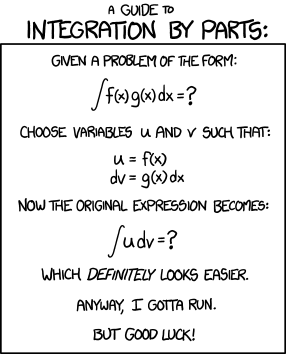
\includegraphics[scale=0.5]{xkcd_ibp.png}
    \caption{Comic from https://xkcd.wtf/1201/}
\end{figure}
\begin{moral}
It is perfectly fine to use integration by parts throughout, but you must be a fool for ignoring all the symmetries..
\end{moral}

In another example, we show that symmetry does not only have to refer to graphical symmetries.

\begin{example}[2021 H3 Math P1/1]
In the diagram, let $R$ be the region between the x-axis and the curve y=$\frac{\ln{x}}{1+x^2}$ for $0\leq x \leq 1$ and let $S$ be the region between the x-axis and the curve $y=\frac{\ln {x}}{1+x^2}$ for $x\geq 1$.
 \begin{figure}[H]
    \centering
    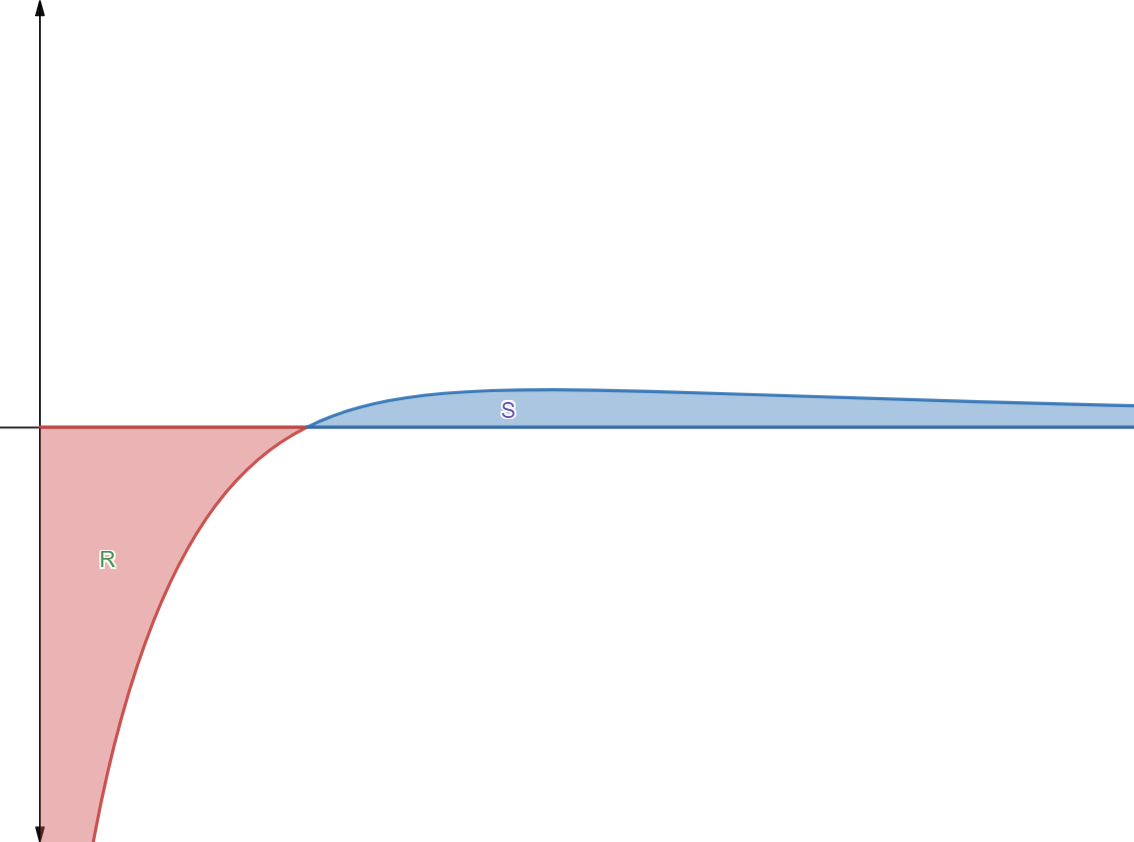
\includegraphics[scale=0.3]{graph-1.PNG}
    \caption{Graph of $y=\frac{\ln{x}}{1+x^2}$}
    \label{fig:1}
\end{figure}
Use the substitution $x=\frac{1}{t}$ to prove that $R$ and $S$ have equal areas.
\end{example}
This part suggests some form of symmetry: I call this the area symmetry. In particular, the question says that, since $R$ and $S$ have equal areas, the integral of the curve for $0 < x \leq 1$ is negative of the integral for $x \geq 1$.

Firstly, the x-intercept is indeed at $x=1$, as suggested from the graph. For  $x=\frac{1}{t}$, $\frac{dx}{dt}=-\frac{1}{t^2}$, and $x=0, t\to \infty$ and $x=1, t=1$. For area $R$, 
\begin{align*}
    \text{area R} &= -\int_0^{1}\frac{\ln{x}}{1+x^2}\,dx \\
    &=-\int_{\infty}^{1}\frac{-\ln{t}}{1+\frac{1}{t^2}} \cdot -\frac{1}{t^2}\,dt\\
    &=\int_{1}^{\infty}\frac{\ln{t}}{t^2+1} \,dt &&\text{by interchanging limits}
\end{align*}
Since $t$ is simply a dummy variable, we may make a switch:
\begin{align*}
    \text{area R} &= -\int_0^{1}\frac{\ln{x}}{1+x^2}\,dx \\
    &=\int_{1}^{\infty}\frac{\ln{x}}{x^2+1} \,dx
\end{align*}
However, this integral for $x\geq 1$ is simply the area of $S$, so we conclude that $R$ and $S$ have equal areas.

\begin{example}[cont.]\label{0.2-subst}
For $a > 0$, use the substitution $x=at$ to find $$\int_{0}^{\infty}\frac{\ln{x}}{a^2+x^2} \,dx.$$
\end{example}
For the choice $x=at$, $\,dx=a\,dt$, so $x=0,t=0$ and $x \to \infty, t\to\infty$.
Thus,
\begin{align*}
    \int_{0}^{\infty}\frac{\ln{x}}{a^2+x^2} \,dx &= a\int_{0}^{\infty}\frac{\ln{at}}{a^2+a^2t^2} \,dt \\
    &= \frac{1}{a}\int_{0}^{\infty}\frac{\ln{a}+\ln{t}}{1+t^2} \,dt \\
    &= \frac{1}{a}\left[\int_{0}^{\infty}\frac{\ln{a}}{1+t^2}\,dt+\int_{0}^{\infty}\frac{\ln{t}}{1+t^2} \,dt\right]
\end{align*}
From the first result, we know that $$\int_{0}^{1}\frac{\ln{t}}{1+t^2} \,dt=-\int_{1}^{\infty}\frac{\ln{t}}{1+t^2} \,dt \Longrightarrow \int_{0}^{\infty}\frac{\ln{t}}{1+t^2} \,dt=0.$$

Hence, we only evaluate the first integral.
\begin{align*}
    \int_{0}^{\infty}\frac{\ln{x}}{a^2+x^2} \,dx
    &= \frac{\ln{a}}{a}\int_{0}^{\infty}\frac{1}{1+t^2}\,dt \\
    &= \frac{\ln{a}}{a}\left[\tan^{-1}{t}\right]_{0}^{\infty} \\
    &= \frac{\ln{a}}{a}\left(\frac{\pi}{2}-1\right)
\end{align*}

\subsection{Selected Problems}
\problem Read up the proofs of the Fundamental Theorem of Calculus and the Mean Value Theorem from a university Calculus textbook.
\problem We refer to the continuation of the pursuit curve setup as in \ref{pursuit-curve:results}.
\begin{enumerate}
    \item Use the substitution $m=\tan\theta$ in \ref{pursuit-curve:results} to deduce the result $m+\sqrt{1+m^2}=\left(1-\frac{x}{D}\right)^{-\lambda}$.
    \item Hence find the explicit equation of the pursuit curve.
\end{enumerate}
\problem Prove the identity in \ref{generalised-quotient-rule:p1}.
\problem* For $a > 0$, use integration by parts to find
$$\int_{0}^{\infty}\ln{\left(\frac{a^2+x^2}{x^2}\right)}\, dx.$$
(Hint: You may like to use the substitution in \nameref{0.2-subst}. Also, the limits may be slightly annoying..)
\problem Find the Maclaurin expansion for $f(x)=x\cot{x}$ up to the first two non-zero terms.
\problem (Generalised Product Rule) Suppose $f$ and $g$ are both $n$-times differentiable functions, then the composition $fg$ is also $n$-times differentiable, and it's $n$-th derivative is given by
$$(fg)^{(n)}=\sum_{k=0}^{n}\binom{n}{k}f^{(n-k)}g^{(k)}.$$
Prove the result by induction.

\problem If $f(x)$ is convex (i.e. $f''(x)>0$, where $f(x)$ is twice-differentiable on the domain $[a,b]$), then \textbf{Jensen's Inequality} implies that $$f\left(\frac{x+y}{2}\right) \leq \frac{f(x)+f(y)}{2}$$
for all $x,y \in [a,b]$.
\begin{enumerate}
    \item Explain this result by considering a sketch (how does a convex function look like?).
    \item* Generalise this result and prove it!
\end{enumerate}

\problem Suppose $f$ is a continuous increasing function and that $f(0)=0$. If $a, b > 0$. 

\begin{enumerate}
    \item *(Young's Inequality) Then, we have $$ab \leq \int_{0}^{a}f(x)\, dx+\int_{0}^{b}f^{-1}(x)\, dx.$$
    Prove this result with the help of a sketch.
    \item Show further that if $p, q > 1$ are such that $\frac{1}{p}+\frac{1}{q}=1$, then
    $$ab \leq \frac{x^p}{p}+\frac{y^q}{q}.$$
    
    Now, define $\{a_i\}_{k=1}^n,\{b_i\}_{k=1}^n$ as two sequences of positive reals and let $x=\sum a_k$, $y=\sum b_k$.
    \item *Show that $$\frac{1}{x^{\frac{1}{p}}y^{\frac{1}{q}}}\sum a_kb_k=\sum\left(\frac{a_k^p}{x}\right)^\frac{1}{p}\left(\frac{b_k^q}{q}\right)^\frac{1}{q}.$$
    \item **(Holder's Inequality) Prove that $$\sum a_kb_k\leq \left(\sum a_k^p\right)^\frac{1}{p}\left(\sum b_k^p\right)^\frac{1}{q}.$$
\end{enumerate} 
\begin{remark}
Holder's Inequality is a generalisation for the Cauchy-Schwarz Inequality. Try to derive it!
\end{remark}

\problem (Lagrange Form of Taylor's Theorem) Suppose $f:[a,x]\to\mathbb{R}$ is $(k+1)$-times differentiable on the interval $(a,x)$. Define, for $t\in (a,x)$
$$F(t)=\sum_{k=0}^{n}\frac{f^{(k)}(t)}{k!}(x-t)^k.$$
Then, there exists $\xi \in (a,x)$ such that
$$f^{(n)}(\xi)=(n+1)!\frac{R(x)}{(x-a)^{n+1}},$$
where $R(x)=F(x)-F(a)$.
\begin{enumerate}
    \item Deduce the Mean Value Theorem.
    \item * Consider the Mean Value Theorem on the rational function $\frac{F'(\xi)}{G'(\xi)}$ for some function $G$ on the domain $[a,b]$. By computing $F'(t)$, find an expression for $R(x)$.
    \item ** Prove the result above by making a suitable choice for $G(t)$.
\end{enumerate}
\begin{remark}
Notice that $R(x)$ is really the remainder(or error) of the approximation of $f$ at the point $x=a$.
\end{remark}
\end{document}